%\let\textcircled=\pgftextcircled
\chapter{Introduction}
\label{chap:intro}

\textbf{Vehicle dynamics reconstruction} is a topic with much interest especially in insurance makers. A car crash can be recreated visually after the event happened. But there are other topics with interest in vehicle dynamics reconstruction, like self-driving vehicles or everything interested in knowing the vehicle position at some point in time. \\
This thesis will analyze techniques for reconstruction based on inertial and GNSS data used in a related software project. \\
In the data collected and used for the project \textbf{inertial} data was created by accelerometers and gyroscopes, while \textbf{GNSS} (Global Navigation Satellite System) by an eletronic receiver. \\ One of the most famous GNSS is the american GPS (Global Positioning System) but during experiments also russian GLONASS and chinese BeiDou signals were received.
All these sensors can be bundled in a box, as in our case, and fitted on a vehicle. \\

\begin{figure}[H]
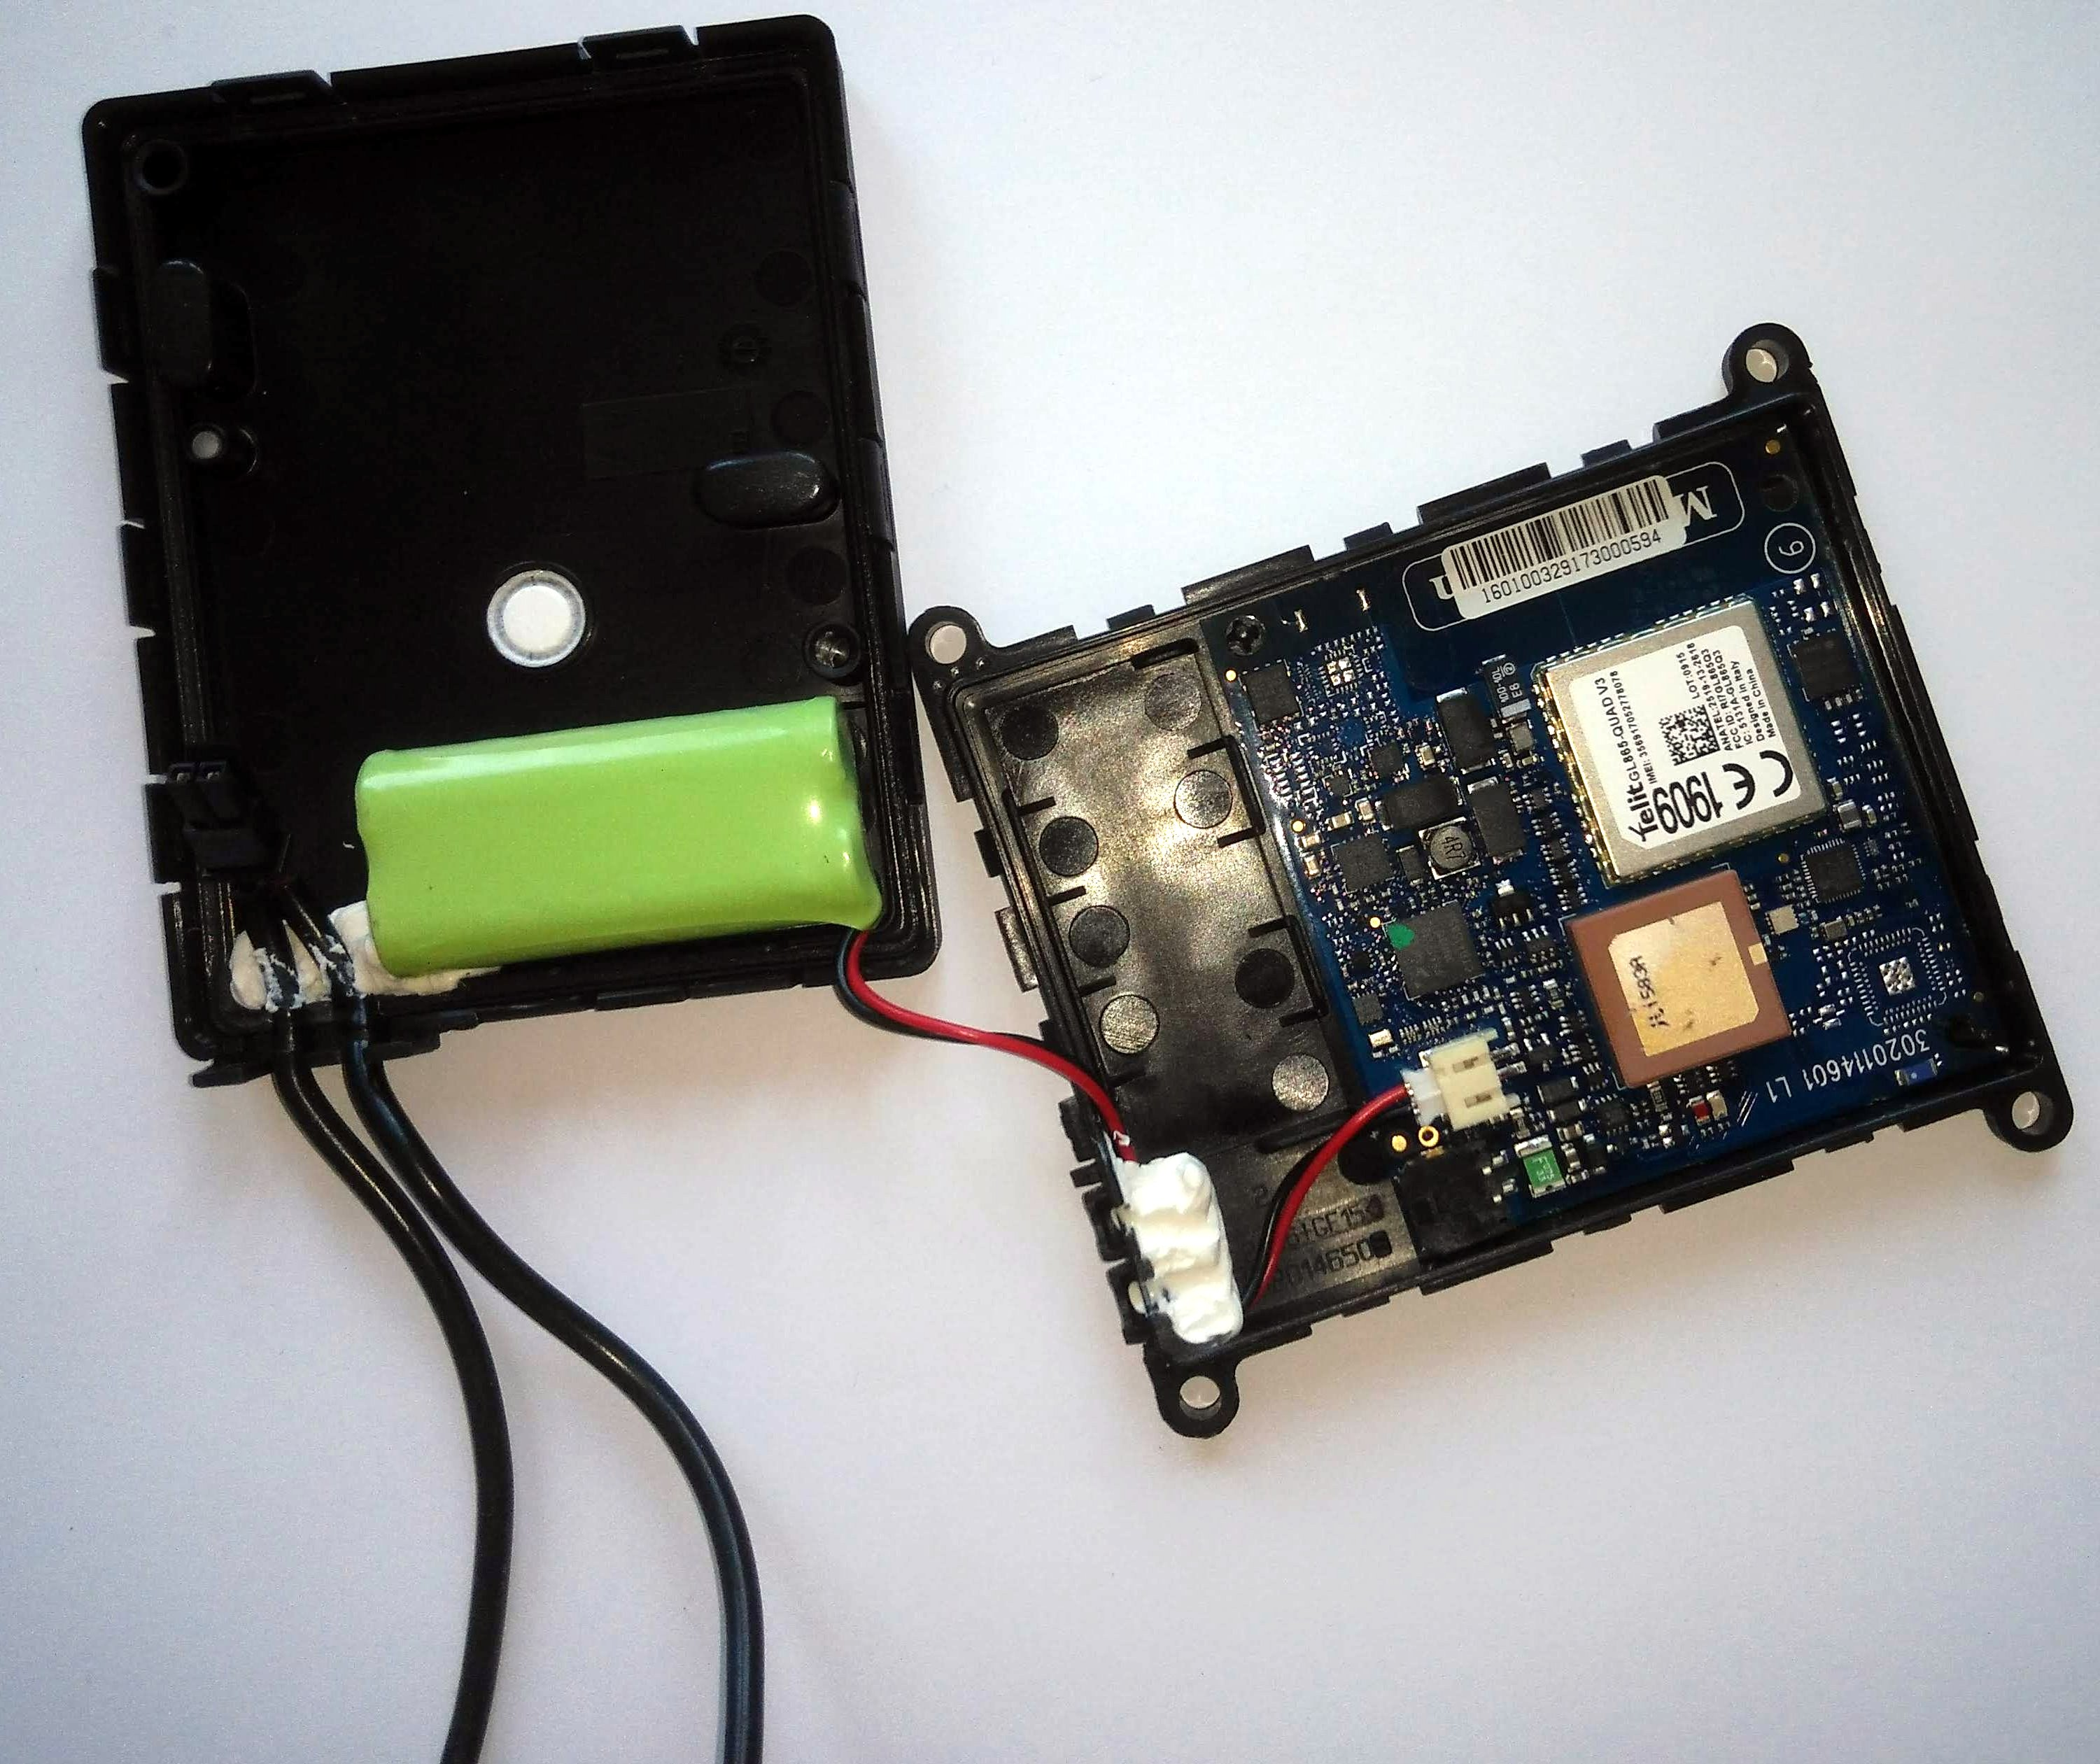
\includegraphics[width=\textwidth]{box.jpg}
\caption{One of the sensor box used to collect data}
\end{figure}

Challenges the aspiring solution may face are: sensor data gathering and transmissoin, correction of bad alignment of sensors, integration numerical error, precision reinforcement with multiple sensor fusion, representation of reconstructed trajectory.

% explain input data and the choose of blender